\documentclass{article}
\usepackage[utf8]{inputenc}
\usepackage[french]{babel}
\usepackage{xcolor}
\usepackage{graphicx}
\usepackage{minted}
\usepackage[TI]{fontenc}

\title{Projet 5}
\author{LEBOBE timothé}
\date{19 juin 2020}

\begin{document}

    \maketitle
    \newpage

    \tableofcontents
    \newpage

    \section{Biographie de Fibonacci}
        Fibonacci est né à Pise mais il étudie en grande partie en Algérie à Bougie, une ville d'influence marchande et intellectuel.
        Il étudie les travaux algébriques du Persan Al-Khwarizmi et de l'Egyptien Abu Kamil. Il voyage beaucoup en aidant son père qui est
        notaire et marchand. Ces voyages lui permettent de rencontrer d'autre mathématiciens. De 1198 à 1228, il compile ses conaissance 
        en écrivant des ouvrages. Après 1228, sa vie est peu connu, en 1241, il a perçut un salaire de la part de la république de Pise
        pour comptabilité. Il meurt peut après.
        \begin{center}
            
\includegraphics{images/Fibonacci_portrait.jpg}
        \end{center}

        \newpage

    \section{La suite de Fibonacci}
        La suite de Fibonacci est exposée dans le livre \textit{liber Abaci} publié en 1202. La suite est montrée comme l'évolution
        d'une population de lapin au cours des mois selon certaines conditions:
        \begin{itemize}
            \item les deux lapins mis dans l'enclos le premier mois sont deux laperaux;
            \item les lapins ne peuvent procréer qu'au 3e mois d'existence;
            \item les lapins en âge de procréer engendre forcément qu'un seul couple de laperaux;
            \item les lapins sont immortels.
        \end{itemize}
        La suite de Fibonacci montre le nombre de couple de lapin.
        \begin{center}
            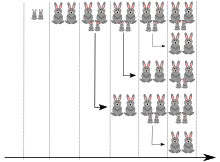
\includegraphics{images/Fibonacci_lapins.png}
        \end{center}
        Dans ce cas, $F_0 = 0; F_1 = 1; F_2 = 1 ;\dots$ \\
        La suite de Fibonacci étant définie par $F_0 = 0; F_1 = 1; F_{n+2} = F_{N+1} + F_n $
        , elle commence par $0, 1, 1, 2, 3, 5, 8, 13, 21, 34, 55$

        \newpage

    \section{Exercie 1: niveau 1}
        \subsection{Enoncé}
            Joseph Marchand prépare ses vacances à la montagne. Comme tous les ans, il va skier. Mais comme tous
            les ans, il doit d’abord vérifier que ses skis sont encore à sa taille.
            D’expérience, il sait qu’il peut porter ses skis même s’il y a quelques tailles de différence avec ses pieds
            (ce qui n’est pas très prudent pour ses chevilles).
            Il vous donne la taille de ses pieds et la taille de ses skis. Pouvez-vous lui donner l’écart entre les deux
            tailles ?
        \subsection{Entrée}
            L’entrée contiendra deux entiers : la taille A des pieds sur la première ligne et la taille B
            des skis sur la seconde.
        \subsection{Sortie}
            Vous afficherez un entier, l’écart constaté entre les deux tailles.
        \subsection{Contraintes}
            \begin{itemize}
                \item $0 <= A <= 10^6$
                \item $0 <= B <= 10^6$
            \end{itemize}
        \subsection{Code}
            \begin{minted}{python}

import re


def diff_taille(a: int, b: int) -> int:
    """function which return the difference between a and b
    ----
    :pre:
        - a is an int and 0 <= a <= 10 ** 6
        - b is an int and 0 <= b <= 10 ** 6
    :post:
        - return_value is an int
    """

    # Assertions pre
    assert isinstance(a, int), \
        "a must be a int, not {}".format(type(a))
    assert 0 <= a <= 10 ** 6, \
        "a must be include between 0 and 10 ** 6, not {}".format(a)
    assert isinstance(b, int), \
        "b must be a int, not {}".format(type(b))
    assert 0 <= b <= 10 ** 6, \
        "b must be include between 0 and 10 ** 6, not {}".format(b)

    # calcul de l'écart
    return_value = (a - b, b - (a + 1))[a < b]

    # Assertion post
    assert isinstance(return_value, int), \
        "return_value must be a int, not {}".format(type(return_value))

    return return_value


# Entrée / inputs
A = input()
while not(re.findall(r"^\d+$", A)) and 0 <= int(A) <= 10 ** 6:
    A = input()
A = int(A)

B = input()
while not (re.findall(r"^\d+$", B)) and 0 <= int(B) <= 10 ** 6:
    B = input()
B = int(B)

# Affichage du résultat
print(diff_taille(A, B))
            \end{minted}
        \newpage

    \section{Exercice 2: niveau 2}
        \subsection{Enoncé}
            Dans son magasin, Joseph Marchand a loué presque tous ses skis, et certaines tailles sont manquantes.
            Cependant, il essaie de répondre aux attentes de chaque nouveau client.
            Lorsqu’un client entre dans le magasin, Joseph lui demande sa taille et parcourt ensuite les paires de skis
            qu’il a à sa disposition pour trouver celle qui correspondrait le mieux. Vous pouvez aider Joseph !
            Ce dernier vous donne la taille d’une paire de skis désirée par un client (notée A ), le nombre de skis qu’il
            a en réserve (noté N), et une liste de la taille de chacun de ces N skis. En échange vous lui donnez la taille
            de la paire de skis de son stock la plus proche de la taille de la paire de skis qui correspond à son client. Si
            plusieurs paires sont à égalité, vous donnerez la plus petite de celles-ci pour économiser du bois ! Il vous en
            sera très reconnaissant.

        \subsection{Entrée}
            L’entrée contiendra trois lignes. La première donnera le nombre de paires de skis en réserve N, la deuxième
            la taille de paire de skis désirée par le client A, et la troisième listera les tailles des paires de skis en stock Si.
        
        \subsection{Sortie}
            Vous afficherez un entier, la taille des skis que la personne devra choisir.
        
        \subsection{Contraintes}
            \begin{itemize}
                \item $1 <= N <= 10 ** 5$
                \item $0 <= A <= 10 ** 9$
                \item $0 <= S_i <= 10 ** 9$
            \end{itemize}

        \subsection{Code}
            \begin{minted}{python}

import re


def client_ski(n: int, a: int, s_i: list) -> int:
    """fonction qui retourne la taille de ski la plus proche de celle que demande le client, en cas d'égalité d'écart, \
    la plus petite est choisie
    ----
    :pre:
        - n est un int appartenant à [0; 10 ** 5]
        - a est un int appartenant à [0; 10 ** 9]
        - s_i est une list de N élements qui appartiennent à [0; 10 ** 9]
    :post:
        - return_value est un int
    """

    # Assertions pre
    assert isinstance(n, int), "n must be a int, not {}".format(type(n))
    assert 0 <= n <= 10 ** 5, "n must be in [0, 10 ** 5], not {}".format(n)
    assert isinstance(a, int), "a must be a int, not {}".format(type(a))
    assert 0 <= a <= 10 ** 9, "a must be in [0, 10 ** 9], not {}".format(a)
    assert isinstance(s_i, list), "s_i must be a list, not {}".format(type(s_i))
    assert len(s_i) == n, "list s_i contain not n element, {} instead of {}".format(len(s_i), n)
    for i,j in enumerate(s_i):
        assert isinstance(j, int), "element {} of s_i must be a int, not {}".format(i, type(j))
        assert 0 <= j <= 10 ** 9, "l'élement {} of s_i must be in [0, 10 ** 9], not {}".format(i, j)

    # le programme initialise les variable par défaut avec la première valeur de la liste
    diff_min = abs(s_i[0] - a)
    return_value = s_i[0]
    # il parcourt la liste, calcule la différence de taille, si la différence est plus petite
    # que la précédente, il met la nouvelle taile de ski et la nouvelle diférence dans les variables
    for i in s_i[1:]:
        dif = abs(i - a)
        if dif < diff_min:
            diff_min = dif
            return_value = i
        elif dif == diff_min and i < return_value:
            return_value = i

    # Assertion post
    assert isinstance(return_value, int), "return_value must be a int, not {}".format(type(return_value))

    return return_value

N = input()
while not(re.findall(r"^\d+$", N)) and 0 <= int(N) <= 10 ** 5:
    N = input()
N = int(N)

A = input()
while not(re.findall(r"^\d+$", A)) and 0 <= int(A) <= 10 ** 9:
    A = input()
A = int(A)

S_i = input()
while not(re.findall("^" + (" ".join([r"\d+"] * N)) + "$", S_i)):
    S_i = input()
S_i = S_i = [int(i) for i in S_i.split(" ")]

print(client_ski(N, A, S_i))

            \end{minted}
        \newpage
        
    \section{Exercice 3: niveau 1}
        \subsection{Enoncé}
            Vous possédez un jeu de pin’s distincts, tous composés d’un engrenage de plusieurs dents dont certaines
            percées d’un trou. Le laboratoire d’Okabé ne cesse de compter de nouveaux membres, et il s’attache à
            distribuer à chacun d’eux un de ces pin’s, en respectant la contrainte suivante : la superposition de deux
            pin’s quelconques doit toujours laisser apparaître un unique trou.
            Ainsi, en cas de glissement dans une dimension parallèle, deux membres quelconques du laboratoire
            pourront toujours se reconnaître en vérifiant que leurs pin’s respectent la propriété.
            On vous demande de vérifier si l’ensemble de pin’s donné respecte bien la contrainte. Il y a N membres
            dans le laboratoire donc N pin’s à vérifier et chacun d’eux comporte M dents possibles dont certaines percées
            d’un trou. On vous garantit que tous les pin’s ont le même nombre de trous.
        
        \subsection{Entrée}
            L’entrée comprendra :
            \begin{itemize}
                \item deux nombres N et M représentant respectivement le nombre de pin’s et le nombre de dents de chaque pin’s.
                \item sur chacune des N lignes suivantes, un pin’s représenté par une chaîne de caractères avec un « o » pour un trou et une espace pour une dent intacte.
            \end{itemize}
        
        \subsection{Sortie}
            Vous devez écrire une ligne sur la sortie standard : 1 si l’ensemble de pin’s respecte la propriété, 0 sinon

        \subsection{Contraintes}
            \begin{itemize}
                \item $1 <= N <= 273$
                \item $1 <= M <= 273$
            \end{itemize}

        \subsection{Code}
            \begin{minted}{python}

import re

def pins_bound(n: int, m: int, s_n: list)-> int:
    """fonction qui retourne 1 si l'ensemble des pin's respecte la propriété de conception du laboratoire Okabé
    ----
    :pre:
        - n est un int et 1 <= n <= 273
        - m est un int et 1 <= n <= 273
        - s_n est une liste de n str
    :post:
        - return_value est un int 0 <= return value <= 1
    """

    # Assertion pre
    assert isinstance(n, int), "n must be a int, not {}".format(type(n))
    assert 1 <= n <= 273, "n must be in [1, 273], not {}".format(n)
    assert isinstance(m, int), "m must be a int, not {}".format(type(m))
    assert 1 <= m <= 273, "m must be in [1, 273], not {}".format(m)
    assert isinstance(s_n, list), "s_n must be a list, not {}".format(type(s_n))
    assert len(s_n) == n, "s_n must have {} elements instead of {} elements".format(n, len(s_n))
    for i, j in enumerate(s_n):
        assert isinstance(j, str), "element {} of s_n must be a str, not {}".format(i, type(j))
        assert len(j) == m, \
            "lengh of element {} is not the same as the first element, {} instead of {}".format(i, len(j, len(s_n[0])))
        assert s_n[0].count("o") == j.count("o"), \
            "there is not the same number of o in the fisrt element as in {} element".format(i)

    # valeur par défaut
    return_value = 1

    places_o = [
        [
            j
            for j in range(len(i))
            if i[j] == 'o'
        ]
        for i in s_n
    ]
    i = 0
    while i < len(places_o) and return_value != 0:
        for j in places_o[i + 1:]:
            bind = 0
            for k in places_o[i]:
                if k in j:
                    bind += 1
            if bind == 0 or bind > 1:
                return_value = 0
        i += 1
    # Assertion post
    assert isinstance(return_value, int), "return_value must be a int, not {}".format(type(return_value))

    return return_value

N_M = input()
while not(re.findall(r"^\d+ \d+$", N_M)) \
    and 1 <= int(N_M.split(" ")[0]) <= 273 \
        and 1 <= int(N_M.split(" ")[1]) <= 273:
    N_M = input("1")
N, M = N_M.split(" ")
N = int(N)
M = int(M)

S_n = []
for i in range(N):
    a = input()
    while not re.findall("^[ o]{" + str(M) + "}$", a):
        a = input(str(i))
    S_n.append(a)

print(pins_bound(N, M, S_n))

            \end{minted}
        \newpage

    \section{Exercice 4: niveau 2}
        \subsection{Enoncé}
            Vous possédez un jeu de clés passe-partout. Ayant minutieusement préparé le cambriolage de cette nuit,
            vous connaissez déjà les caractéristiques des serrures auxquelles vous allez vous attaquer (ancienneté et niveau
            de sécurité) et les limites de vos passe-partout : un passe-partout est dit de force (xi
            , yi) s’il peut ouvrir les
            serrures datées d’avant 1990 (aussi dites « traditionnelles ») de sécurité au plus xi et les serrures datées de
            1990 ou après (aussi dites « rectifiées ») de sécurité au plus yi.
            Vous savez, de votre longue expérience de cambrioleur professionnel, que le temps de l’opération est un
            facteur décisif : pas question donc de trimbaler toutes sortes de clés inutiles. Vous cherchez à savoir le nombre
            minimal de passe-partout à emporter pour pouvoir ouvrir toutes les serrures. S’il est impossible de toutes les
            ouvrir avec votre ensemble de clés, retournez 0.
        
        \subsection{Entrée}
            L'entrée comprendra:
            \begin{itemize}
                \item un nombre N, le nombre de passe-partout que vous possédez ;
                \item sur chacune des N lignes suivantes, deux nombres xi et yi , représentant la force de votre i-ème passepartout ;
                \item un nombre M, le nombre de serrures que vous comptez cambrioler ;
                \item sur chacune des M lignes suivantes, deux nombres ai et si, correspondant respectivement à l’ancienneté de la serrure (-1 pour « avant 1990 », 1 pour « 1990 ou après ») et au niveau de sécurité de la i-ème serrure.
            \end{itemize}
        
        \subsection{Sortie}
            Vous afficherez en sortie :
            \begin{itemize}
                \item le nombre minimum de passe-partout à emporter pour mener à bien votre tâche si c’est possible, 0 sinon.
            \end{itemize}

        \subsection{Contraintes}
            \begin{itemize}
                \item $1 <= N <= 1 000$;
                \item $1 <= M <= 100 000$;
                \item $1 <= xi, yi, si <= 1 000 000$
            \end{itemize}
        
        \subsection{Code}
            \begin{minted}{python}

def pass_partout(n: int, m: int, s_p_p: list, portes: list)-> int:
    """fonction qui retourne 0 si toutes les portes ne peuvent pas être ouverte
    sinon le nombre de clé minimum nécessaire
    ----
    :pre:
        - n est un int et 1 <= u <= 10 ** 3
        - m est un int et 1 <= m <= 10 ** 5
        - s_p_p est une list de n tuples \
            d'entier et 1 <= x_i, y_i <= 10 ** 9
        - portes est une list de m tuples \
            d'entier et 1 <= s_i <= 10 ** 9\
                et -1 == a_i ou 1 == a_i
    :post:
        - return_value est un int et 0 <= return_value <= 2
    """

    # Assertion pre
    assert isinstance(n, int), \
        "n must be a int, not {}".format(type(n))
    assert 1 <= n <= 10 ** 3, \
        "n must be in [1, 10 ** 3], not {}".format(n)
    assert isinstance(m, int), \
        "m must be a int, not {}".format(type(m))
    assert 1 <= m <= 10 ** 5, \
        "m must be in [1, 10 ** 5], not {}".format(m)
    assert isinstance(s_p_p, list), \
        "s_p_p must be a list, not {}".format(type(m))
    for i, j in enumerate(s_p_p):
        assert isinstance(j, tuple), \
            "element {} of s_p_p must be a tuple, not {}".format(i, type(j))
        assert len(j) == 2, \
            "element {} of s_p_p must have a lengh of 2, not {}".format(i, len(j))
        for k, l in enumerate(j):
            assert isinstance(l, int), \
                "element {} of element {} of s_p_p must be a int, not {}".format(k, i, type(l))
            assert 1 <= l <= 10 ** 9, \
                "element {} of element {} of s_p_p must be in [1, 10 ** 9], not {}".format(k, i, l)
    for i, j in enumerate(portes):
        assert isinstance(j, tuple), \
            "element {} of portes must be a tuple, not {}".format(i, type(j))
        assert len(j) == 2, \
            "element {} of portes must have a lengh of 2, not {}".format(i, len(j))
        for k, l in enumerate(j):
            assert isinstance(l, int), \
                "element {} of element {} of portes must be a int, not {}".format(k, i, type(l))
        assert -1 <= j[0] <= 1, \
            "element 0 of element {} of portes must be in [-1, 1], not {}".format(i, j[0])
        assert 1 <= j[1] <= 10 ** 9, \
            "element 1 of element {} of portes must be in [1, 10 ** 9], not {}".format(i, j[1]) 

    # variables
    return_value = 0
    open_door = 0

    # le programme détermine le meilleur passe partout pour chacun des 2 type de porte
    # le programme met le premier passe-partout comme valeur de départ
    best_pp_o, best_pp_n = [s_p_p[0]] * 2

    for i in s_p_p[1:]:
        x_i, y_i = i
        if x_i > best_pp_o[0]:
            best_pp_o = i
        if y_i > best_pp_n[1]:
            best_pp_n = i

    for porte in portes:
        porte: tuple
        age, level_door = porte
        # si la porte est d'avant 1990 et si la porte est ouvrable
        if (age == -1 and best_pp_o[0] >= level_door) \
            or (age == 1 and best_pp_n[0] >= level_door):
            open_door += 1

    if open_door == m:
        if best_pp_n == best_pp_o:
            return_value = 1
        else:
            return_value = 2

    assert isinstance(return_value, int), \
        "return_value must be a int, not {}".format(type(return_value))

    return return_value

N = input()
while not re.findall(r"^\d+$", N) and 1 <= int(N) <= 10 ** 3:
    N = input()
N = int(N)
passes_partout = []
for i in range(N):
    passe_partout = input()
    while not(re.findall(r"^\d+ \d+$", passe_partout)) \
        and 1 <= int(passe_partout.split(" ")[0]) <= 10 ** 6 \
            and 1 <= int(passe_partout.split(" ")[0]) <= 10 ** 6:
        passe_partout = input()
    passes_partout.append(passe_partout.split(" "))
del passe_partout

M = input()
while not(re.findall(r"^\d+$", M)) and 1 <= int(M) <= 10 ** 6:
    M = input()
M = int(M)

Portes = []
for i in range(M):
    porte = input()
    while not(re.findall(r"^1 \d+$|^-1 \d+$", porte)) and (-1 == porte.split(" ")[0] or 1 == porte.split(" ")[0]) \
        and 1 <= porte.split(" ")[1] <= 10 ** 6:
        porte = input()
    Portes.append(porte.split(" "))
print(pass_partout(N, M, passes_partout, Portes))

            \end{minted}
        \newpage

\end{document}
